\chapter{对称性与守恒律}

\problem{对于时间和广义坐标的任意函数\(F(t,\bm{q})\),证明其时间全导数\(\frac{\dd F}{\dd t}\)自动满足欧拉-拉格朗日方程,即其对应的运动方程恒为零。}

\begin{solution}
	证明只需作计算即可。记\(\dot{F}:=\frac{\dd F}{\dd t}\),那么
	\[\dot{F}=\frac{\dd F}{\dd t}=\frac{\partial F}{\partial t}+\frac{\partial F}{\partial q^a}\dot{q}^a\]
	计算
	\[\frac{\partial \dot{F}}{\partial q^a}=\frac{\partial^2 F}{\partial q^a\partial t}+\frac{\partial^2 F}{\partial q^a\partial q^b}\dot{q}^b\]
	\[\frac{\partial \dot{F}}{\partial \dot{q}^a}=\frac{\partial F}{\partial q^a}\]
	\[\frac{\dd}{\dd t}\frac{\partial \dot{F}}{\partial \dot{q}^a}=\frac{\partial^2 F}{\partial t\partial q^a}+\frac{\partial^2 F}{\partial q^a\partial q^b}\dot{q}^b\]
	考虑到偏导数可交换次序,可知
	\[\frac{\partial \dot{F}}{\partial q^a}-\frac{\dd}{\dd t}\frac{\partial \dot{F}}{\partial \dot{q}^a}=0\]
	恒成立,证毕。
	
	此题也可以从最小作用量原理来证明,将\(L=\frac{\dd F}{\dd t}\)代入得到
	\[S=\int_{t_1}^{t_2} L \dd t=\int_{t_1}^{t_2} \frac{\dd F}{\dd t} \dd t=F(t_2,\bm{q}(t_2))-F(t_1,\bm{q}(t_1))\]
	固定\(\bm{q}(t_1)\)和\(\bm{q}(t_2)\),那么上式右端是个常数,变分为零,自然满足欧拉-拉格朗日方程。
\end{solution}



\problem{单自由度系统的拉格朗日量为\(L=L(t,q,\dot{q})\)。(1)证明运动方程方程可以具体写成\(\frac{\partial^2 L}{\partial \dot{q}^2}\ddot{q}+\frac{\partial^2 L}{\partial q\partial \dot{q}}\dot{q}+\frac{\partial^2 L}{\partial t\partial \dot{q}}-\frac{\partial L}{\partial q}=0\);(2)若将\(L\)换成全导数\(\frac{\dd F}{\dd t}\),证明其自动满足(1)中的运动方程,即是恒等式。据此说明若两个拉格朗日量\(L\)和\(\tilde{L}\)相差时间全导数,即有\(\tilde{L}-L=\frac{\dd F}{\dd t}\),则给出相同的运动方程。}

\begin{solution}
	(1)欧拉-拉格朗日方程为
	\[\frac{\dd }{\dd t}\frac{\partial L}{\partial \dot{q}}-\frac{\partial L}{\partial q}=0\]
	使用链式法则即得
	\[\frac{\dd }{\dd t}\frac{\partial L}{\partial \dot{q}}=\frac{\partial^2 L}{\partial t\partial \dot{q}}+\frac{\partial^2 L}{\partial q\partial \dot{q}}\frac{\dd q}{\dd t}+\frac{\partial^2 L}{\partial \dot{q}^2}\frac{\dd \dot{q}}{\dd t}\]
	由于\(\frac{\dd q}{\dd t}=\dot{q},\frac{\dd \dot{q}}{\dd t}=\ddot{q}\),即得
	\[\frac{\partial^2 L}{\partial \dot{q}^2}\ddot{q}+\frac{\partial^2 L}{\partial q\partial \dot{q}}\dot{q}+\frac{\partial^2 L}{\partial t\partial \dot{q}}-\frac{\partial L}{\partial q}=0\]
	
	(2)证明在5.1题已经做过了,此处略。由此可知若\(\tilde{L}=L+\frac{\dd F}{\dd t}\),那么
	\[\frac{\partial \tilde{L}}{\partial q}-\frac{\dd }{\dd t}\frac{\partial \tilde{L}}{\partial \dot{q}}=\frac{\partial L}{\partial q}-\frac{\dd}{\dd t}\frac{\partial L}{\partial \dot{q}}+\frac{\partial \dot{F}}{\partial q}-\frac{\dd}{\dd t}\frac{\partial \dot{F}}{\partial \dot{q}}=\frac{\partial L}{\partial q}-\frac{\dd}{\dd t}\frac{\partial L}{\partial \dot{q}}\]
	也就是说,它们能给出相同的运动方程。
\end{solution}



\problem{某系统广义坐标为\(q\),已知其拉格朗日量为\(L=a\dot{q}^2+b\dot{q}^3\ddot{q}+c\ddot{q}q^3+d\ddot{q}\dot{q}q^2\),其中\(a,b,c,d\)都是常数。求与\(L\)相差时间全导数的、不含广义加速度\(\ddot{q}\)的等价拉格朗日量\(\tilde{L}\)。}

\begin{solution}
	推导只需反复分离全微分即可。
	
	对于\(a\dot{q}^2\)项,不含\(\ddot{q}\)。
	
	对于\(b\dot{q}^3\ddot{q}\)项,分部积分得到
	\[\dot{q}^3\ddot{q}=\frac{\dd }{\dd t}(\dot{q}^4)-3\dot{q}^3\ddot{q}\]
	即\(b\dot{q}^3\ddot{q}=\frac{1}{4}\frac{\dd }{\dd t}(b\dot{q}^4)\)。
	
	对于\(c\ddot{q}q^3\)项,分部积分得到
	\[\ddot{q}q^3=\frac{\dd}{\dd}(q^3 \dot{q})-3 q^2 \dot{q}^2\]
	即\(c\ddot{q}q^3=-3c q^2 \dot{q}^2+\frac{\dd}{\dd t}(c q^3 \dot{q})\)。
	
	对于\(d\ddot{q}\dot{q}q^2\)项,分部积分得到
	\begin{align*}
		\ddot{q}\dot{q}q^2&=\frac{\dd}{\dd t}(q^2 \dot{q}^2)-\dot{q}\frac{\dd}{\dd t}(q^2 \dot{q})\\
		&=-q^2\dot{q}\ddot{q}-2 q \dot{q}^3+\frac{\dd}{\dd t}(q^2 \dot{q}^2)\\
		2 \ddot{q}\dot{q}q^2&=-2 q \dot{q}^3+\frac{\dd}{\dd t}(q^2 \dot{q}^2)\\
		\ddot{q}\dot{q}q^2 &=-q \dot{q}^3+\frac{\dd}{\dd t}(\frac{1}{2}q^2 \dot{q}^2)
	\end{align*}
	即\(d\ddot{q}\dot{q}q^2=-d q \dot{q}^3+\frac{\dd}{\dd t}(\frac{1}{2}d q^2 \dot{q}^2)\)
	
	综合上述式子,得到
	\begin{align*}
		L&=a\dot{q}^2+b\dot{q}^3\ddot{q}+c\ddot{q}q^3+d\ddot{q}\dot{q}q^2\\
		&=a\dot{q}^2-3c q^2 \dot{q}^2-d q \dot{q}^3+\frac{\dd}{\dd t}(b\dot{q}^4+c q^3 \dot{q}+\frac{1}{2}d q^2 \dot{q}^2)
	\end{align*}
	与\(L\)相差时间全导数的、不含广义加速度\(\ddot{q}\)的等价拉格朗日量\(\tilde{L}\)为
	\[\tilde{L}=a\dot{q}^2-3c q^2 \dot{q}^2-d q \dot{q}^3\]
\end{solution}



\problem{已知质量\(m=1\)的一维谐振子拉格朗日量为\(L=\frac{1}{2}\dot{q}^2-\frac{1}{2}\omega^2 q^2\),考虑拉格朗日量\(\tilde{L}=\frac{1}{12}\dot{q}^4+\frac{\omega^2}{2}q^2 \dot{q}^2-\frac{\omega^4}{4}q^4\)。(1)证明\(L\)运动方程的解也是\(\tilde{L}\)的运动方程的解;(2)证明\(\tilde{L}\)不能表达成\(\tilde{L}=L+\frac{\dd F(t,q)}{\dd t}\)的形式。}

\begin{solution}
	(1)由欧拉-拉格朗日方程
	\[\frac{\partial L}{\partial q}-\frac{\dd}{\dd t}\frac{\partial L}{\partial \dot{q}}=0\]
	得到运动方程为\(\ddot{q}+\omega^2 q=0\)。对于\(\tilde{L}\)则为
	\[\frac{\partial \tilde{L}}{\partial q}-\frac{\dd}{\dd t}\frac{\partial \tilde{L}}{\partial \dot{q}}=0\]
	代入得到
	\[-\omega^4 q^3+\omega^2 q\dot{q}^2-\dot{q}^2\ddot{q}-\omega^2\frac{\dd }{\dd t}(q^2\dot{q})=0\]
	\[-\omega^4 q^3+\omega^2 q\dot{q}^2-\dot{q}^2\ddot{q}-\omega^2(q^2\ddot{q}+2q\dot{q}^2)=0\]
	整理为
	\[-\omega^2 q^2(\omega^2 q+\ddot{q})-\dot{q}^2(\omega^2 q+\ddot{q})=0\]
	\[-(\omega^2 q^2+\dot{q}^2)(\omega^2 q+\ddot{q})=0\]
	由于\(\omega^2 q^2+\dot{q}^2=0\)当且仅当\(q(t)=0\),此时\(q(t)\)同时满足两个方程,其余情况消去\(\omega^2 q^2+\dot{q}^2\),两个运动方程的解相同。
	
	(2)显然,由于
	\[\frac{\dd F(t,q)}{\dd t}=\frac{\partial F(t,q)}{\partial t}+\frac{\partial F(t,q)}{\partial q}\dot{q}\]
	其中只含有\(\dot{q}\)的一次项,但是\(\tilde{L}\)中含有\(\dot{q}\)的四次项,等式也就不能成立了。
\end{solution}



\problem{利用广义坐标和广义速度的变换关系,证明 (5.37)。}

\begin{solution}
	书中式(5.37)是如下的式子:
	\[\frac{\dd }{\dd t}\frac{\partial\tilde{L}}{\partial\dot{\tilde{q}}^a}-\frac{\partial\tilde{L}}{\partial \dot{\tilde{q}}^a}=\frac{\partial q^b}{\partial \tilde{q}^a}\left(\frac{\dd}{\dd t}\frac{\partial L}{\partial\dot{q}^b}-\frac{\partial L}{\partial q^b}\right)\]
	正文中给出了从最小作用量原理的推导过程,此处直接验证。
	
	待施工.
\end{solution}



\problem{已知一维谐振子的拉格朗日量为\(L=\frac{1}{2}m\dot{q}^2-\frac{1}{2}m\omega^2 q^2\),利用运动方程,证明\(C(t,q,\dot{q})=\arctan{\frac{\omega q}{\dot{q}}}-\omega t\)是运动常数。}

\begin{solution}
	由欧拉-拉格朗日方程得到运动方程为
	\[\ddot{q}+\omega^2 q=0\]
	对\(C(t,q,\dot{q})\)求导得到
	\[\frac{\dd C(t,q,\dot{q})}{\dd t}=\frac{\frac{\omega\dot{q}^2-\omega q \ddot{q}}{\dot{q}^2}}{1+\left(\frac{\omega q}{\dot{q}}\right)^2}-\omega=\frac{\omega\dot{q}^2-\omega q \ddot{q}}{\omega^2 q^2+\dot{q}^2}-\omega=\frac{\omega\dot{q}^2-\omega q \ddot{q}-\omega(\omega^2 q^2+\dot{q}^2)}{\omega^2 q^2+\dot{q}^2}=-\frac{\omega q(\ddot{q}+\omega^2 q)}{\omega^2 q^2+\dot{q}^2}=0\]
	因此\(C(t,q,\dot{q})=\arctan{\frac{\omega q}{\dot{q}}}-\omega t\)是运动常数,证毕。
\end{solution}



\problem{考虑例(2.9)中光滑细杆上的小球,如图\ref{fig:5-7}所示,假设细管放在光滑水平面上,且绕一端以恒定角速度\(\omega\)旋转。(1)选取合适的广义坐标,写出粒子的拉格朗日量并求其运动方程;(2)求粒子的能量函数\(h\),并分析其是否是运动常数;(3)粒子的能量函数\(h\)和总能量\(E=T+V\)相等吗?为什么?(4)粒子的总能量\(E=T+V\)是运动常数吗?尝试解释原因。}
\begin{figure}[h]
	\centering
	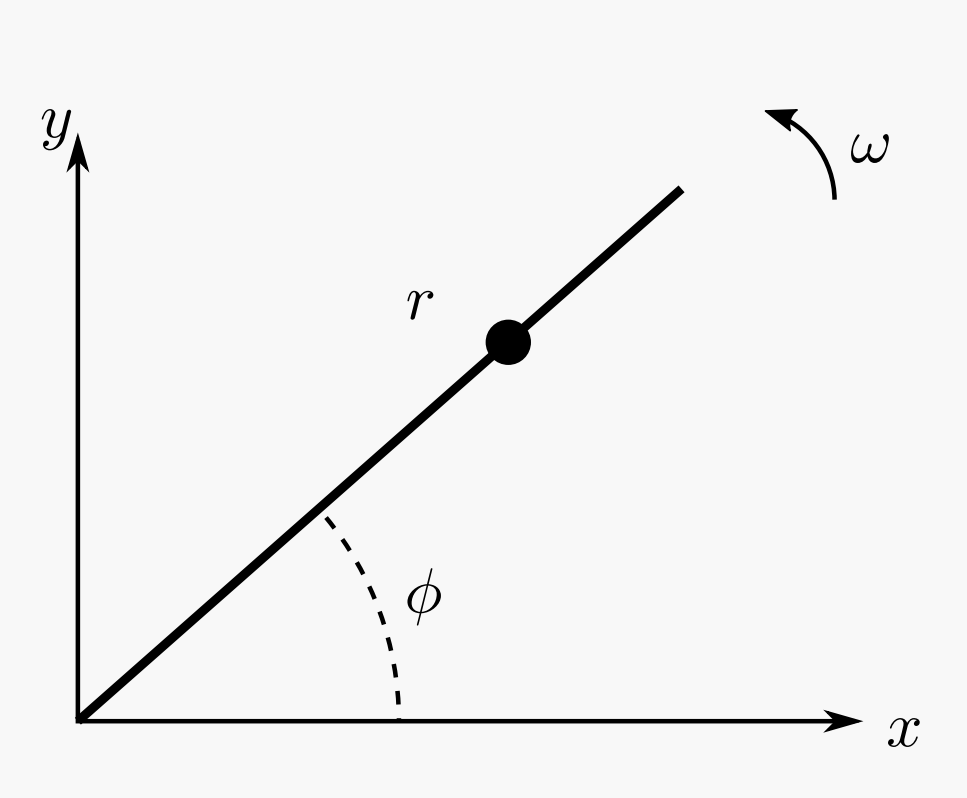
\includegraphics[width=0.3\textwidth]{content/Figures/5-7}
	\caption{ }
	\label{fig:5-7}
\end{figure}
	
\begin{solution}
	待施工.
\end{solution}



\problem{}
\begin{solution}
	待施工.
\end{solution}



\problem{}
\begin{solution}
	待施工.
\end{solution}



\problem{}
\begin{solution}
	待施工.
\end{solution}



\problem{}
\begin{solution}
	待施工.
\end{solution}



\problem{}
\begin{solution}
	待施工.
\end{solution}



\problem{}
\begin{solution}
	待施工.
\end{solution}



\problem{}
\begin{solution}
	待施工.
\end{solution}



\problem{}
\begin{solution}
	待施工.
\end{solution}



\problem{}
\begin{solution}
	待施工.
\end{solution}



\problem{}
\begin{solution}
	待施工.
\end{solution}


